\section{Preliminaries}\label{sec:preliminaries}

The later computations replace a boundary-dynamics problem by finite data from
the facets of a polytope.  This section fixes the common language needed for
that passage: action and contact normalization, the EHZ capacity and systolic
ratio, normalized facet data and Lagrangian products, and finally Clarke's
position-free dual problem.  The next section will specialize these objects to
polytopes and prove that the capacity problem contains a finite pure-facet
minimizer.

All convex bodies below are compact convex subsets of \(\mathbb{R}^4\) with
non-empty interior. Unless stated otherwise, the origin lies in the interior.

\subsection{Convex and symplectic notation}\label{subsec:preliminaries-polytopes}

We write \(\mathbb{R}^4\) with coordinates \((q_1,q_2,p_1,p_2)\). The standard
complex structure is
\[
  J_0 =
  \begin{pmatrix}
    0 & -I_2 \\
    I_2 & 0
  \end{pmatrix},
\]
and the standard symplectic form is
\[
  \omega_0(u,v) = \langle J_0u,v\rangle
  = \sum_{i=1}^2 (u_{q_i}v_{p_i}-u_{p_i}v_{q_i}).
\]
We will use \(J_0^2=-I\), \(J_0^{\mathsf T}=-J_0\), and
\(\omega_0(J_0u,J_0v)=\omega_0(u,v)\) without further comment.
We use the standard primitive
\[
  \lambda_0 = \frac{1}{2}\sum_{i=1}^2(q_i\,dp_i-p_i\,dq_i).
\]
Thus \(d\lambda_0=\omega_0\) and
\(\lambda_0|_x(v)=\frac12\langle -J_0v,x\rangle\).
Thus, for an absolutely continuous closed curve
\(\gamma\colon[0,T]\to\mathbb{R}^4\), its action is
\begin{equation}\label{eq:preliminaries-action}
  A(\gamma) \coloneqq \int_\gamma \lambda_0
  = \frac{1}{2}\int_0^T
    \langle -J_0\dot{\gamma}(t),\gamma(t)\rangle\,dt.
\end{equation}
This action is invariant under orientation-preserving reparametrization.

\begin{lemma}[Symplectic shoelace formula]\label{lem:preliminaries-shoelace}
Let \(z\colon[0,T]\to\mathbb{R}^4\) be a closed piecewise affine curve. Suppose
that \(z\) has constant velocity \(w_k\) on consecutive intervals of length
\(\ell_k\), for \(k=1,\ldots,m\). Then
\begin{equation}\label{eq:preliminaries-shoelace}
  2A(z)
  =
  \sum_{1\leq j<k\leq m}
    \ell_j\ell_k\,\omega_0(w_j,w_k).
\end{equation}
In particular, the action of a closed pure-word Reeb orbit depends only on the
cyclic velocity word and the dwell times, not on the base point.
\end{lemma}

\begin{proof}
Write \(t_k=\sum_{j<k}\ell_j\). On the \(k\)-th interval,
\[
  z(t)=z(0)+\sum_{j<k}\ell_jw_j+(t-t_k)w_k.
\]
The contribution of \(z(0)\) to
\(\int_0^T\langle -J_0\dot z,z\rangle\,dt\) vanishes because \(z\) is closed,
so \(\sum_k\ell_kw_k=0\). The self-term
\(\langle -J_0w_k,w_k\rangle\) vanishes by skew-symmetry. Hence
\[
  2A(z)
  =
  \sum_k
    \ell_k\left\langle -J_0w_k,\sum_{j<k}\ell_jw_j\right\rangle
  =
  \sum_{j<k}\ell_j\ell_k\,\omega_0(w_j,w_k),
\]
using \(\omega_0(u,v)=\langle J_0u,v\rangle\).
\end{proof}


\subsection{Convex Hamiltonians}
\label{subsec:preliminaries-convex-hamiltonian-language}

The smooth characteristic line field has a convex-analytic formulation that
continues to make sense when \(\partial K\) is not smooth.  For a convex body
\(K\) containing the origin, its support and gauge functions are
\[
  h_K(y)\coloneqq\max_{x\in K}\langle x,y\rangle,
  \qquad
  g_K(x)\coloneqq\inf\{r>0:x\in rK\}.
\]
The boundary is the level set \(g_K=1\).  We use the convex,
\(2\)-homogeneous Hamiltonian
\[
  H_K(x)\coloneqq g_K(x)^2.
\]
For a convex function \(H\), its subdifferential at \(x\) is
\[
  \partial H(x)
  =\{y:H(z)\geq H(x)+\langle y,z-x\rangle
    \text{ for every }z\}.
\]
When \(H\) is differentiable, this set consists only of \(\nabla H(x)\).

\begin{definition}[Contact-normalized generalized characteristic]
\label{def:preliminaries-generalized-characteristic}
A \emph{contact-normalized generalized characteristic} on \(\partial K\) is
a curve \(\gamma\in W^{1,2}([0,T],\mathbb R^4)\), with \(T>0\) and
\(\gamma(0)=\gamma(T)\), whose image lies in \(\partial K\) and which satisfies
\begin{equation}\label{eq:preliminaries-generalized-characteristic}
  -J_0\dot\gamma(t)\in\partial H_K(\gamma(t))
  \quad\text{for almost every }t\in[0,T].
\end{equation}
\end{definition}

For smooth \(K\), the subdifferential in
\eqref{eq:preliminaries-generalized-characteristic} is the singleton
\(\{\nabla H_K\}\).  The resulting Hamiltonian vector is tangent to the
characteristic line on \(\partial K\).  Thus the definition recovers the Reeb
orbits described above, including their parametrization.
\begin{figure}[htbp]
  \centering
  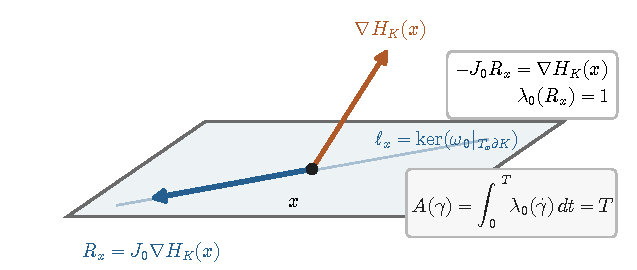
\includegraphics[width=0.94\linewidth]
    {figures/foundations/characteristic-normalization.pdf}
  \caption{The characteristic and contact normalizations at a smooth boundary
  point.  This is a dimension-reduced tangent-space schematic: it records that
  \(R_x=J_0\nabla H_K(x)\) spans the characteristic line inside
  \(T_x\partial K\), but projected angles and lengths carry no meaning.  The
  contact condition \(\lambda_0(R_x)=1\) turns elapsed time into action.}
  \label{fig:preliminaries-characteristic-normalization}
\end{figure}

The normalization also persists without smoothness.  Indeed, if
\(y\in\partial H_K(x)\), then the \(2\)-homogeneity of \(H_K\) gives
\[
  \langle y,x\rangle=2H_K(x).
\]
Along a generalized characteristic, \(H_K(\gamma)=1\), and hence
\[
  \lambda_0|_{\gamma(t)}(\dot\gamma(t))
  =\frac12\langle-J_0\dot\gamma(t),\gamma(t)\rangle
  =1
  \quad\text{for almost every }t.
\]
Consequently every contact-normalized generalized characteristic satisfies
\begin{equation}\label{eq:preliminaries-generalized-characteristic-action-period}
  A(\gamma)=T.
\end{equation}

This formulation separates the general nonsmooth dynamical object from its
finite description on a polytope.  The latter will follow by calculating the
subdifferential of \(H_K\) from the active facets.

\subsection{EHZ capacity}\label{subsec:preliminaries-smooth-symplectic-geometry}

For smooth convex bodies, the Ekeland--Hofer and Hofer--Zehnder capacities
coincide. The common value is the least action needed to close up a
characteristic trajectory on the boundary. We use the resulting EHZ capacity in
the form
\begin{equation}\label{eq:preliminaries-ehz-capacity}
  c_{\mathrm{EHZ}}(K)
  = \min\{A(\gamma):\gamma
    \text{ is a closed characteristic on }\partial K\}.
\end{equation}
Equivalently, the minimum may be taken over Reeb orbits. The contact
normalization only chooses the parametrization of each characteristic, while
the action is a line integral and is invariant under orientation-preserving
reparametrization. For a contact-normalized representative, \(A(\gamma)\) is
also the period. The minimum exists and is positive; for the thesis we use this
standard existence result as background \cite{Rabinowitz1978}. For nonsmooth
convex bodies, and in particular for polytopes, the same capacity is obtained
by approximation and by minimizing over the generalized characteristics of
Definition~\ref{def:preliminaries-generalized-characteristic}. Their finite
facet description on a polytope is derived in
Section~\ref{sec:generalized-reeb-orbits-polytopes}.

As a symplectic capacity on convex bodies, \(c_{\mathrm{EHZ}}\) is monotone
under inclusion, invariant under symplectomorphisms, and conformal:
\[
  c_{\mathrm{EHZ}}(\lambda K)=\lambda^2c_{\mathrm{EHZ}}(K)
  \quad(\lambda>0).
\]
It is normalized by
\[
  c_{\mathrm{EHZ}}(B^4(r))=c_{\mathrm{EHZ}}(Z^4(r))=\pi r^2,
\]
where \(B^4(r)\) is the radius-\(r\) ball and
\(Z^4(r)=B^2(r)\times\mathbb{R}^2\) is the symplectic cylinder. These axioms
are used only as background; the finite computations below use the
minimum-action and quadratic-program descriptions.

Throughout the thesis, \(\operatorname{vol}_4\) denotes four-dimensional
Lebesgue measure in the coordinate order \((q_1,q_2,p_1,p_2)\). In dimension
four we measure the normalized capacity-to-volume ratio by
\begin{equation}\label{eq:preliminaries-systolic-ratio}
  \operatorname{sys}(K)
  \coloneqq
  \frac{c_{\mathrm{EHZ}}(K)^2}{2\operatorname{vol}_4(K)}.
\end{equation}
With this normalization, Viterbo's conjecture for four-dimensional convex
bodies says
\[
  \operatorname{sys}(K)\leq 1,
  \qquad\text{equivalently}\qquad
  c_{\mathrm{EHZ}}(K)^2\leq 2\operatorname{vol}_4(K)
\]
\cite{Viterbo2000}. Later sections use
\(\operatorname{sys}\) for this ratio for polytopes as well, via the same
capacity value discussed above.

\begin{definition}[Systolic-ratio symmetries]
\label{def:preliminaries-systolic-ratio-symmetries}
Let
\[
  G_{\operatorname{sys}}
  =
  \{x\mapsto b+\rho Mx:
    b\in\mathbb R^4,\ \rho>0,\ M\in\operatorname{Sp}(4,\mathbb R)\}.
\]
This is the group of affine transformations generated by translations,
positive scalings, and linear symplectic transformations.
\end{definition}

\begin{lemma}[Systolic-ratio invariance]
\label{lem:preliminaries-systolic-ratio-invariance}
For every convex body \(K\subset\mathbb R^4\) and every
\(g\in G_{\operatorname{sys}}\),
\[
  \operatorname{sys}(gK)=\operatorname{sys}(K).
\]
\end{lemma}

\begin{proof}
Translations and linear symplectic transformations are symplectomorphisms, so
they preserve \(c_{\mathrm{EHZ}}\). They also preserve four-dimensional
volume, because translations do not change volume and every symplectic matrix
has determinant \(1\). A positive scaling by \(\rho\) gives
\[
  c_{\mathrm{EHZ}}(\rho K)=\rho^2c_{\mathrm{EHZ}}(K),
  \qquad
  \operatorname{vol}_4(\rho K)=\rho^4\operatorname{vol}_4(K).
\]
Substituting these identities in
\eqref{eq:preliminaries-systolic-ratio} shows that the ratio is unchanged.
\end{proof}

This is a geometric symmetry group acting on unlabelled convex bodies. In a
labelled coordinate chart, the same unlabelled body may also be represented
after relabelling facets or inequalities; that relabelling ambiguity is a
coordinate issue, not an additional element of \(G_{\operatorname{sys}}\).

\begin{proposition}[Continuity]\label{prop:preliminaries-sys-hausdorff-continuity}
Let \(K_t\) be a family of four-dimensional convex bodies which is continuous
in the Hausdorff topology. Then \(c_{\mathrm{EHZ}}(K_t)\) is continuous in
\(t\). If, moreover, \(t\mapsto\operatorname{vol}_4(K_t)\) is positive,
finite, and continuous, then the systolic ratio of the family is continuous.
\end{proposition}

\begin{proof}
The EHZ capacity is \(C^0\)-continuous on convex bodies with respect to the
Hausdorff metric \cite{CH2021}. The assertion for \(\operatorname{sys}\) is
then ordinary continuity of the quotient in
\eqref{eq:preliminaries-systolic-ratio}. In the applications below the volume
hypothesis is usually automatic, since four-volume is continuous under
Hausdorff convergence of convex bodies; for the rotated-polygon family it is
even constant.
\end{proof}

\subsection{Polytope input language}
\label{subsec:preliminaries-polytope-input-language}

The finite methods represent polytopes by normalized halfspaces. Let
\(K\subset\mathbb R^4\) be full-dimensional with
\(0\in\operatorname{int}(K)\). We write
\begin{equation}\label{eq:preliminaries-normalized-halfspaces}
  K=\{x\in\mathbb R^4:\langle a_i,x\rangle\leq1,
    \ i=1,\ldots,F\}.
\end{equation}
If \(n_i\) is the outward unit normal to the corresponding supporting
hyperplane and \(h_i=h_K(n_i)>0\) is its height, then
\[
  a_i=\frac{n_i}{h_i}.
\]
For an irredundant description, the vectors \(a_i\) are precisely the vertices
of the polar body
\[
  K^\circ=\operatorname{conv}\{a_1,\ldots,a_F\}.
\]

\begin{figure}[htbp]
  \centering
  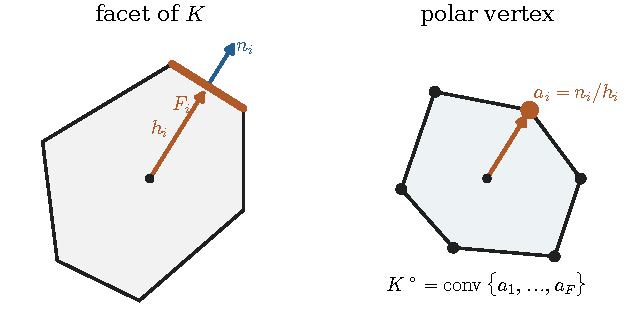
\includegraphics[width=0.92\linewidth]
    {figures/foundations/facet-polarity.pdf}
  \caption{Facet normalization and polarity in a planar model.  The
  supporting line \(\langle n_i,x\rangle=h_i\) becomes
  \(\langle a_i,x\rangle=1\) after setting \(a_i=n_i/h_i\), and that row is a
  vertex of the polar polygon.  The same facet--polar-vertex correspondence
  holds in four dimensions; the planar metric proportions are specific to
  this example and are not part of the duality statement.}
  \label{fig:preliminaries-facet-polarity}
\end{figure}

Conversely, the normalized halfspaces define a bounded full-dimensional
polytope containing the origin in its interior exactly when
\(0\in\operatorname{int}\operatorname{conv}\{a_i\}\).  The description is
irredundant exactly when the listed vectors are pairwise distinct and every
\(a_i\) is an extreme point of this convex hull.

The ordered list \((a_1,\ldots,a_F)\) is a labelled presentation.  Relabelling
the same inequalities does not change the unlabelled convex body, but labels
matter when an algorithm records facet words or when a local calculation uses
the \(a_i\) as coordinates.

\subsection{Lagrangian products}
\label{subsec:preliminaries-lagrangian-products}

Write
\[
  \mathbb R^4=\mathbb R_q^2\oplus\mathbb R_p^2
  =\{(q_1,q_2,p_1,p_2)\}.
\]
\begin{definition}[Lagrangian product]
\label{def:preliminaries-lagrangian-product}
For planar convex bodies \(K_q,K_p\subset\mathbb R^2\), their Lagrangian
product is
\begin{equation}\label{eq:preliminaries-lagrangian-product}
  K_q\times_L K_p
  =\{(q_1,q_2,p_1,p_2):(q_1,q_2)\in K_q,\ (p_1,p_2)\in K_p\}.
\end{equation}
Thus \(K_q\) occupies the Lagrangian \(q\)-plane and \(K_p\) occupies the
Lagrangian \(p\)-plane.  This is different from taking a product of planar
domains in the symplectic coordinate planes \((q_1,p_1)\) and \((q_2,p_2)\).
\end{definition}

The central examples of the thesis are Lagrangian products of polygons; their
lifted facet rows and the resulting restricted word enumeration are introduced
with the Haim--Kislev formula, where they are first used.

\subsection{Clarke dual action principle}\label{subsec:preliminaries-clarke-dual-action-principle}

The finite Haim--Kislev formula used in
Section~\ref{sec:quadratic-program-algorithm-hk2019} rests on a dual
variational viewpoint. The literature often states this connection in a fixed
\([0,1]\)-period normalization. We use a free-period normalization instead:
the dual curves below have period \(T\), satisfy \(A(z)=T\), and are not
centered by a condition such as \(\int z=0\). Translation is handled as a
symmetry, not as a constraint. This is equivalent to the normalized formulation
used by Haim--Kislev, but the numerical equalities below are written in the
free-period convention used throughout this thesis.

\begin{lemma}[Fenchel duality for the gauge]\label{lem:preliminaries-fenchel-duality}
The Legendre--Fenchel conjugate of \(g_K^2\) is
\(\frac{1}{4}h_K^2\). Equivalently,
\[
  g_K^2(x) + \frac{1}{4}h_K^2(y) \geq \langle x,y\rangle
\]
for all \(x,y\in\mathbb{R}^4\), with equality if and only if
\[
  y\in \partial g_K^2(x)
  \quad\Longleftrightarrow\quad
  x\in \partial\bigl(\tfrac{1}{4}h_K^2\bigr)(y).
\]
\end{lemma}

\begin{proof}
For fixed \(y\), write \(x=\lambda u\) with \(\lambda\geq0\) and
\(g_K(u)=1\). Since \(g_K(\lambda u)^2=\lambda^2\),
\[
  (g_K^2)^*(y)
  = \sup_{\lambda\geq0}
      \sup_{g_K(u)=1}\{\lambda\langle u,y\rangle-\lambda^2\}
  = \sup_{\lambda\geq0}\{\lambda h_K(y)-\lambda^2\}
  = \frac{1}{4}h_K(y)^2.
\]
The Fenchel inequality and the equality/subdifferential condition are the
standard equality cases for a convex function and its conjugate.
\end{proof}

Define the dual functional on absolutely continuous closed curves
\[
  z\colon[0,T]\to\mathbb{R}^4
\]
by
\begin{equation}\label{eq:preliminaries-dual-functional}
  I_K(z) \coloneqq
  \frac{1}{4}\int_0^T h_K^2(-J_0\dot{z}(t))\,dt.
\end{equation}
The dual problem is
\begin{equation}\label{eq:preliminaries-dual-problem}
  \min\{I_K(z):
    z\in W^{1,2}([0,T],\mathbb{R}^4),\;
    z(0)=z(T),\; T>0,\; A(z)=T\}.
\end{equation}

\begin{definition}[Weak dual critical curve]\label{def:preliminaries-weak-dual-critical}
A closed curve
\[
  z\in W^{1,2}([0,T],\mathbb{R}^4),
  \qquad A(z)=T,
\]
is \emph{weak dual critical} if there are
\(\nu\in\mathbb{R}\) and \(b\in\mathbb{R}^4\) such that
\begin{equation}\label{eq:preliminaries-dual-euler-lagrange}
  \nu z(t)+b
  \in \partial\bigl(\tfrac{1}{4}h_K^2\bigr)(-J_0\dot{z}(t))
  \quad\text{for a.e. }t.
\end{equation}
Equivalently,
\[
  -J_0\dot{z}(t)\in\partial g_K^2(\nu z(t)+b)
  \quad\text{for a.e. }t.
\]
\end{definition}

We use one general result from Clarke's nonsmooth variational theory:
minimizers of the dual action functional exist, and the nonsmooth Lagrange
multiplier rule applies to the action constraint \cite[Ch.~5]{Clarke1983}.
For nonsmooth convex bodies this is the variational input used by
Artstein--Avidan--Ostrover and Haim--Kislev
\cite[Propositions~2.5, 2.7 and Lemmas~5.1, 5.2]{AAO2014}
\cite[Section~2]{HK2017}.

Those sources state the dual problem in a fixed-\([0,1]\) normalization, with
closed loops \(w\) satisfying \(A(w)=\frac12\). The passage to the free-period
normalization above is by explicit rescaling. If \(z\) is defined on \([0,T]\)
and satisfies \(A(z)=T\), then
\[
  w(s)=\frac{1}{\sqrt{2T}}\,z(Ts)
\]
satisfies \(A(w)=\frac12\) and \(I_K(w)=I_K(z)/2\). Conversely, if \(w\) is a
fixed-period dual curve and \(c=2I_K(w)\), then
\[
  z(t)=\sqrt{2c}\,w(t/c),
  \qquad 0\leq t\leq c,
\]
satisfies \(A(z)=c\) and \(I_K(z)=c\). Under the same rescaling, the fixed-period
weak-critical equation used by Haim--Kislev becomes
\eqref{eq:preliminaries-dual-euler-lagrange}. If a cited version fixes the
translation freedom by imposing a centering condition on \(w\), this is only a
choice of representative: \(A\), \(I_K\), and the weak-critical equation are
translation-invariant after adjusting the constant \(b\). Thus the cited
analytic input is the fixed-period existence and weak-criticality theorem; the
rest of this subsection writes out the convention translation and Reeb
correspondence in the free-period, uncentered notation used here.

\begin{lemma}[Euler--Lagrange equation in thesis convention]
\label{lem:preliminaries-dual-euler-lagrange}
Every minimizer of the dual problem is weak dual critical in the sense of
Definition~\ref{def:preliminaries-weak-dual-critical}.
\end{lemma}

\begin{proof}
Let \(z\) be a minimizer of the free-period dual problem, and rescale it to the
fixed-\([0,1]\) curve \(w\) above. The fixed-period Clarke theorem gives the
nonsmooth Euler--Lagrange inclusion for \(w\), with one multiplier for the
constraint \(A(w)=\frac12\). Rescaling this inclusion back to \([0,T]\) gives
the same equation for \(z\). We spell out the resulting equation in the
free-period notation.

There is \(\alpha\in\mathbb{R}\) such that \(z\) satisfies the nonsmooth
Euler--Lagrange inclusion for
\[
  L(z,\dot z)
  =\frac14h_K^2(-J_0\dot z)
    +\alpha\langle -J_0\dot z,z\rangle.
\]
Thus there is an absolutely continuous \(\xi\) with
\[
  \xi(t)\in\partial_{\dot z}L(z(t),\dot z(t)),
  \qquad
  \dot\xi(t)=\nabla_z L(z(t),\dot z(t)).
\]
The right-hand side is \(-\alpha J_0\dot z\). On the left-hand side, the chain
rule for \(\frac14h_K^2(-J_0\dot z)\) gives
\[
  \partial_{\dot z}L
  =J_0\,\partial\bigl(\tfrac14h_K^2\bigr)(-J_0\dot z)
    +\alpha J_0z.
\]
Hence there is
\(p(t)\in\partial(\frac14h_K^2)(-J_0\dot z(t))\) with
\[
  J_0\dot p+\alpha J_0\dot z=-\alpha J_0\dot z.
\]
Since \(J_0\) is invertible, \(\dot p=-2\alpha\dot z\), and therefore
\[
  p(t)=b-2\alpha z(t)
\]
for some constant \(b\in\mathbb{R}^4\). With \(\nu=-2\alpha\), this is exactly
\eqref{eq:preliminaries-dual-euler-lagrange}. The equivalent formulation
follows from Lemma~\ref{lem:preliminaries-fenchel-duality}.
\end{proof}

\begin{lemma}[Scaling and translation]\label{lem:preliminaries-dual-symmetry}
Let \(z\) be weak dual critical on \([0,T]\). For every
\(\alpha>0\) and every \(b\in\mathbb{R}^4\), the curve
\[
  z'(t)=\alpha z(t/\alpha^2)+b,
  \qquad 0\leq t\leq \alpha^2T,
\]
is again weak dual critical. Moreover
\[
  A(z')=\alpha^2A(z)=\alpha^2T,
  \qquad
  I_K(z')=I_K(z).
\]
\end{lemma}

\begin{proof}
Closure is immediate. The action identity follows by substituting
\(s=t/\alpha^2\); the term containing the constant vector \(b\) integrates to
zero because \(z\) is closed. For the dual functional,
\[
  I_K(z')
  =\frac{1}{4}\int_0^{\alpha^2T}
    h_K^2\!\left(-\frac{1}{\alpha}J_0\dot{z}(t/\alpha^2)\right)\,dt
  =I_K(z),
\]
using the \(1\)-homogeneity of \(h_K\). The Euler--Lagrange inclusion is
preserved because
\(\partial(\frac14 h_K^2)(\lambda y)=\lambda
\partial(\frac14 h_K^2)(y)\) for \(\lambda>0\).
\end{proof}

\begin{theorem}[Clarke dual action principle in free-period form]\label{thm:preliminaries-clarke-dual-action}
For a smooth convex body \(K\), and for polytopes after interpreting closed
characteristics as generalized Reeb orbits in the sense of
Section~\ref{sec:generalized-reeb-orbits-polytopes}, the primal minimum and the
dual minimum \eqref{eq:preliminaries-dual-problem} agree:
\[
  c_{\mathrm{EHZ}}(K)
  = \min_\gamma A(\gamma)
  = \min_z I_K(z).
\]
More precisely, every contact-normalized closed characteristic is weak dual
critical, and every weak dual critical curve has a translate/rescale in the
sense of Lemma~\ref{lem:preliminaries-dual-symmetry} that is a
contact-normalized closed characteristic.
\end{theorem}

\begin{proof}
Let \(\gamma\) be a contact-normalized closed characteristic of period \(T\).
Then \(g_K^2(\gamma)=1\),
\(-J_0\dot{\gamma}\in\partial g_K^2(\gamma)\), and \(A(\gamma)=T\). By
Lemma~\ref{lem:preliminaries-fenchel-duality},
\[
  \gamma(t)\in
  \partial\bigl(\tfrac{1}{4}h_K^2\bigr)(-J_0\dot{\gamma}(t))
  \quad\text{for a.e. }t.
\]
This is the dual Euler--Lagrange condition with \(\nu=1\) and \(b=0\).
Thus \(\gamma\) is weak dual critical, and
Lemma~\ref{lem:preliminaries-dual-symmetry} gives the whole
translate/rescale family.

Conversely, let \(z\) be weak dual critical of period \(T\). Choose
\(\nu,b\) as in Definition~\ref{def:preliminaries-weak-dual-critical}. The
equivalent inclusion in that definition gives
\[
  -J_0\dot{z}(t)\in\partial g_K^2(\nu z(t)+b).
\]
The multiplier \(\nu\) is nonzero. If \(\nu=0\), then closedness of \(z\) and
convexity would imply \(0\in\partial g_K^2(b)\), hence \(b=0\), and then the
dual Euler--Lagrange condition would force \(\dot{z}=0\), contradicting
\(A(z)=T>0\).

Set \(x(t)=\nu z(t)+b\). For almost every \(t\), the chain rule for the convex
function \(g_K^2\) gives
\[
  \frac{d}{dt}g_K^2(x(t))
  = \langle -J_0\dot{z}(t),\nu\dot{z}(t)\rangle
  =0.
\]
Since \(z\) is closed, \(g_K^2(x(t))\) is constant; write
\(g_K(x(t))=c>0\). Integrating the Fenchel equality gives
\[
  c^2T+I_K(z)
  =\int_0^T\langle x(t),-J_0\dot{z}(t)\rangle\,dt
  =2\nu A(z)=2\nu T.
\]
The left-hand side is positive, so \(\nu>0\).

Define
\[
  \gamma(t)=\frac{\nu z(t/\nu)+b}{c},
  \qquad 0\leq t\leq \nu T.
\]
Then \(g_K(\gamma)=1\). Using the \(2\)-homogeneity of \(g_K^2\),
\(\partial g_K^2(x/c)=c^{-1}\partial g_K^2(x)\), so
\[
  -J_0\dot{\gamma}(t)
  =-\frac{1}{c}J_0\dot{z}(t/\nu)
  \in \partial g_K^2(\gamma(t)).
\]
Thus \(\gamma\) is a contact-normalized closed characteristic. A direct action
computation gives
\[
  A(\gamma)=\frac{\nu^2}{c^2}A(z)=\frac{\nu^2}{c^2}T.
\]
Since \(\gamma\) is contact-normalized, \(A(\gamma)=\nu T\). Hence
\(\nu=c^2\), and
\[
  \gamma(t)=c\,z(t/c^2)+\frac{b}{c},
\]
so \(\gamma\) lies in the translate/rescale family of \(z\).

It remains to compare the values. For any contact-normalized closed
characteristic \(\gamma\), Fenchel equality gives
\[
  g_K^2(\gamma)+\frac{1}{4}h_K^2(-J_0\dot{\gamma})
  =\langle \gamma,-J_0\dot{\gamma}\rangle.
\]
After integration,
\[
  T+I_K(\gamma)=2A(\gamma)=2T.
\]
Thus \(I_K(\gamma)=T=A(\gamma)\). The value \(I_K\) is constant on the
translate/rescale family by Lemma~\ref{lem:preliminaries-dual-symmetry}.
Conversely, the argument above sends every weak dual critical curve to a
contact-normalized closed characteristic in its translate/rescale family.
Therefore the infima over contact-normalized closed characteristics and over
weak dual critical curves agree. The nonsmooth existence part of Clarke's
principle gives a minimizer of the dual problem, and
Lemma~\ref{lem:preliminaries-dual-euler-lagrange} shows that such a minimizer
is weak dual critical. Hence the dual minimum is attained among the curves just
considered, and the primal and dual minima agree.
\end{proof}

The point of the theorem is not just the equality of two numbers. The primal
formulation constrains a curve to lie on \(\partial K\) and to satisfy a
differential inclusion. The dual formulation removes the position constraint
and makes the functional depend only on \(\dot{z}\). In their equivalent
fixed-period normalization, Haim--Kislev exploit this freedom to choose a
capacity minimizer on a polytope with a finite, simple facet-word description
\cite{HK2017}.

